\documentclass[border=4pt]{standalone}
% Shared typography and colours for the standalone figures.
\usepackage{unicode-math}
\setmainfont{TeX Gyre Termes}
\setmathfont{TeX Gyre Termes Math}
\usepackage{tikz}
\usetikzlibrary{arrows.meta,positioning,calc,decorations.pathreplacing}
\usepackage{pgfplots}
\pgfplotsset{compat=1.18}
\definecolor{elemA}{HTML}{1F5FA8}
\definecolor{elemB}{HTML}{B8461B}
\definecolor{elemC}{HTML}{2E7D32}
\definecolor{elemD}{HTML}{6A4C93}
\definecolor{frameline}{HTML}{555555}

\begin{document}
\begin{tikzpicture}
\begin{axis}[width=12cm,height=6.6cm,xmin=0,xmax=1.18,ymin=0,ymax=2.2,
 axis lines=left,xlabel={$t$ (s)},ylabel={$-w$ (V)},xtick={0,.5,1},ytick={0,1,2},
 legend style={at={(.03,.97)},anchor=north west,draw=none,font=\small},
 clip=false]
\addplot[elemA,thick,dashed,domain=0:1,samples=2] {2*x};
\addlegendentry{ideal compensation}
\addplot[elemC,very thick,domain=0:1,samples=151] {2*(x-.1*(1-exp(-10*x)))};
\addlegendentry{finite actuator}
\node[anchor=west,font=\small,elemA] at (axis cs:1.02,2.04) {$2$};
\node[anchor=west,font=\small,elemC] at (axis cs:1.02,1.72) {$\dfrac{9+e^{-10}}5$};
\end{axis}
\end{tikzpicture}
\end{document}
